\documentclass{article}
\usepackage{color}
\usepackage{amsmath}
\usepackage{tikz}
\usetikzlibrary{arrows}
\usetikzlibrary{calc}
\usepackage{pgfplots}
\pgfplotsset{compat=1.17}

\begin{document}

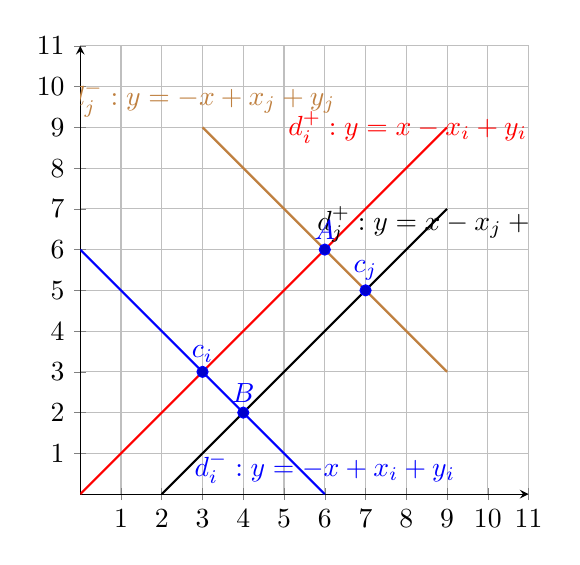
\begin{tikzpicture}
   \begin{axis}
   [axis x line=bottom,axis y line = left, 
   grid = major,
   axis equal image,
   ytick = {1,2,3,4,5,6,7,8,9,10,11},
   xtick = {1,2,3,4,5,6,7,8,9,10,11},
   xmin=0,
   xmax=11,
   ymin=0,
   ymax=11,
   nodes near coords,
   point meta=explicit symbolic]
   \addplot+[only marks] coordinates{(3,3)[$c_i$] (7,5)[$c_j$] (4,2)[$B$] (6,6)[$A$]};
    \addplot+[mark = none, red, thick] coordinates{(0,0) (9,9)} node[xshift = -0.5cm] {$d^+_i: y = x - x_i + y_i$};
    \addplot+[mark = none, blue, thick] coordinates{(0,6) (6,0)} node[above,pos=1] {$d^-_i: y = - x + x_i + y_i$};
    \addplot+[mark = none, thick] coordinates{(2,0) (9,7)} node[xshift = -0.1cm, yshift = -0.2cm] {$d^+_j: y = x - x_j + y_j$};
     \addplot+[mark = none, color = brown, thick] coordinates{(9,3) (3,9)} node[above,pos=1] {$d^-_j: y = - x + x_j + y_j$};
    \end{axis}
    \end{tikzpicture}

\end{document}